% ===== s05_results =====
\section{Results and Analysis}
Table~\ref{tab:main} and Fig.~\ref{fig:results} report the held-out test results. Every value is from a single run with seed 42; no confidence intervals or significance tests were computed, so small differences should not be over-interpreted.

\begin{table}[!t]
\centering
\caption{Test-set results (single run, seed 42). Best value per column in bold.}
\label{tab:main}
\footnotesize
\begin{tabular}{@{}lcccc@{}}
\toprule
\textbf{Model} & \textbf{Macro-F1} & \textbf{ROC-AUC} & \textbf{FPR} & \textbf{Time (ms)} \\
\midrule
Logistic regression & 0.6905 & 0.6937 & 0.6109 & $<$res. \\
Random forest & 0.8562 & 0.9274 & \textbf{0.2015} & 0.0156 \\
XGBoost & 0.8975 & 0.9467 & 0.2375 & 0.0019 \\
LightGBM & \textbf{0.9106} & \textbf{0.9467} & 0.2526 & 0.0182 \\
Compact MLP & 0.6904 & 0.7135 & 0.6115 & 0.0006 \\
MLP, top-3 features & 0.6796 & 0.6401 & 0.6330 & $<$res. \\
\bottomrule
\end{tabular}
\end{table}

\begin{figure*}[!t]
\centering
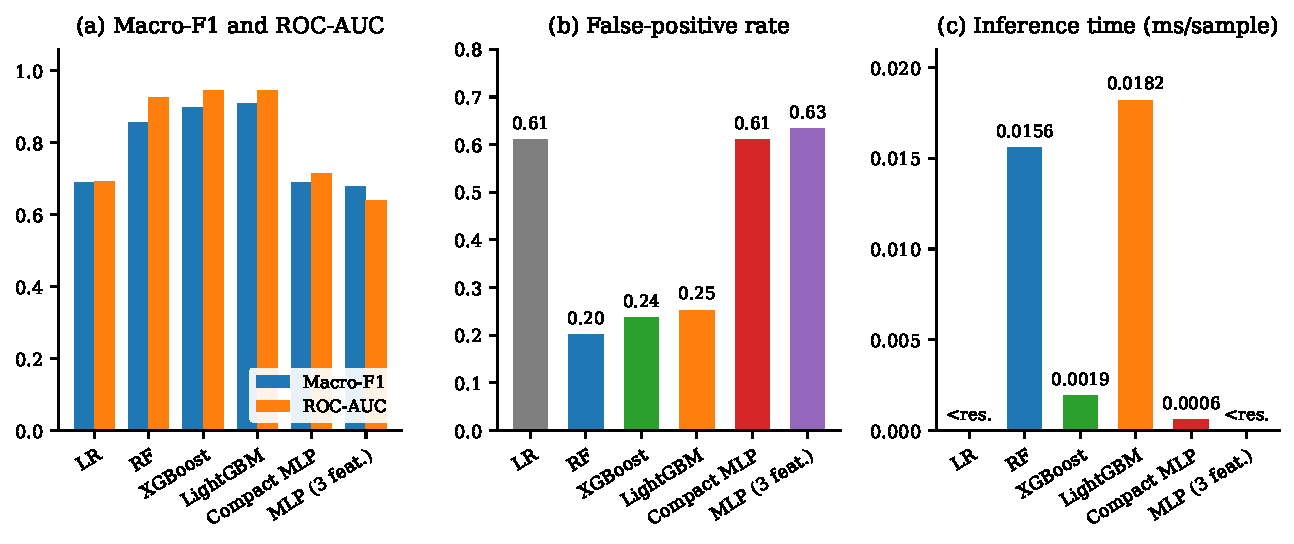
\includegraphics[width=0.95\textwidth]{figures/fig_results.pdf}
\caption{Test-set comparison: (a) macro-F1 and ROC-AUC, (b) false-positive rate, (c) inference time per sample (values below the timer resolution are marked ``$<$res.'').}
\label{fig:results}
\end{figure*}

\textbf{Tree ensembles versus the compact MLP.} LightGBM improves on the compact MLP by 0.2203 in macro-F1, 0.2332 in ROC-AUC, and lowers the FPR by 0.3589 (Table~\ref{tab:main}). XGBoost and LightGBM have ROC-AUC values that differ by about $9\times10^{-6}$, which is not a meaningful difference. The compact MLP matches logistic regression almost exactly (macro-F1 0.6904 versus 0.6905; FPR 0.6115 versus 0.6109), and its training loss fell only from 0.4998 at epoch 5 to 0.4868 at epoch 20, suggesting that it behaves as a near-linear model under this preprocessing.

\textbf{False positives.} All models raise many false alarms: the lowest FPR is 0.2015 (random forest), and the MLP and logistic regression flag about 61\% of benign flows. With benign traffic a small minority, such rates would produce a large share of false alerts in operation.

\textbf{Cost.} The MLP's inference time (0.0006\,ms per sample) is about 24 times lower than random forest's, 28 times lower than LightGBM's, and 3 times lower than XGBoost's. These timings use wall-clock batch prediction with coarse resolution and no repetitions, so only the order of magnitude is reliable.

\subsection{SHAP Feature Analysis}
Fig.~\ref{fig:shap} shows the ten highest-ranked features of the random forest. \texttt{orig\_ip\_bytes} (about 0.19 mean $|\phi|$), \texttt{duration} (about 0.145), and \texttt{orig\_pkts} (about 0.098) lead the ranking, followed by the unnamed leading column (about 0.082), then \texttt{history\_C}, \texttt{conn\_state\_S0}, \texttt{conn\_state\_OTH}, \texttt{proto\_udp}, \texttt{history\_S}, and \texttt{orig\_bytes}, all below 0.015 (values read from the figure). Volume and duration features thus dominate, and the Zeek state \texttt{S0} (connection attempt with no reply) is consistent with scanning behaviour. The prominence of the index column is a warning sign, discussed in Section~VIII.

\begin{figure}[!t]
\centering
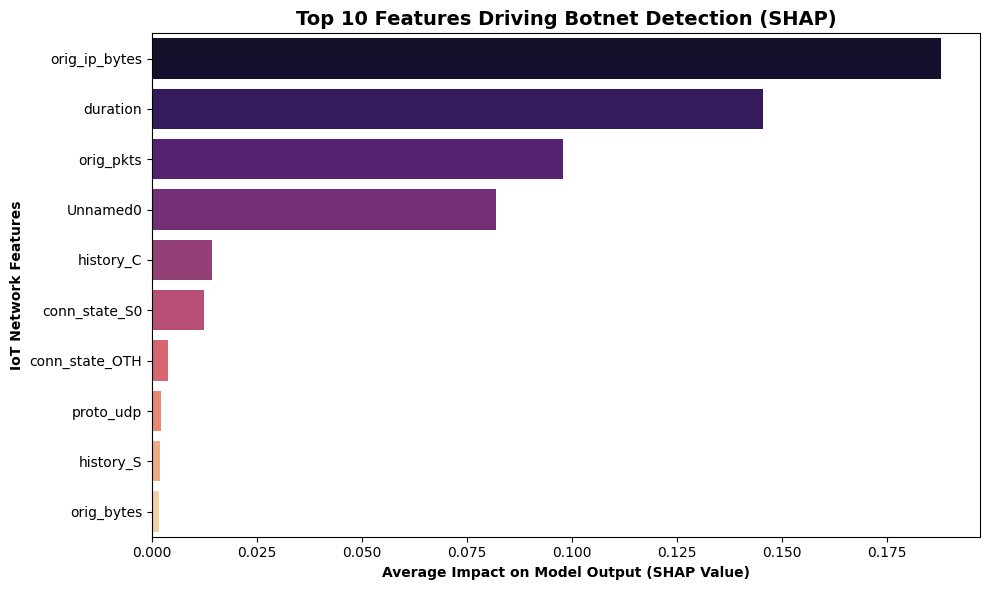
\includegraphics[width=\columnwidth]{figures/nb_cell4.png}
\caption{Top-10 SHAP features of the random forest (mean absolute SHAP value, attack class, 1,000 test flows). \texttt{Unnamed0} is the residual unnamed leading column (apparently a row index).}
\label{fig:shap}
\end{figure}